\documentclass{article} % For LaTeX2e
\usepackage{iclr2019_conference,times}
\usepackage{times}
\usepackage{helvet}
\usepackage{courier}
\usepackage{graphicx}
\usepackage{hyperref}
\usepackage{url}
\usepackage{graphicx}
\usepackage{amsmath}
\usepackage{amsfonts}
\usepackage{todonotes}
\usepackage{epstopdf}
\usepackage{color}
\usepackage{verbatim}
\usepackage{pdfpages}
\usepackage{ amssymb }
\usepackage{caption}
\usepackage{subcaption}
\usepackage{float}
 \usepackage{booktabs}
 \usepackage{colortbl}
 \usepackage{tabularx}

% \renewcommand{\arraystretch}{1.2}
%\frenchspacing

\title{Classification of Cheatgrass Invasion using Biophysical and Remote Sensing Data}

\author{Aaron Tuor  \& Kyle Larson \\
Pacific Northwest National Laboratory\\
\texttt{\{aaron.tuor, kyle.larson\}@pnnl.gov}}

\newcommand{\fix}{\marginpar{FIX}}
\newcommand{\new}{\marginpar{NEW}}
\newcommand\crule[3][black]{\textcolor{#1}{\rule{#2}{#3}}}

%\iclrfinalcopy % Uncomment for camera-ready version, but NOT for submission.
\begin{document}
    \maketitle

\begin{abstract} 
In this study we explore machine learning approaches to help land managers map the presence of the invasive exotic annual grass, cheatgrass ({\em Bromus tectorum}), which is dramatically altering wildfire regimes in the Western United States and threatening environmental sustainability and human life. 
We investigate different data fusion strategies of integrating biophysical data (e.g., soils, climate, solar radiation) and remotely sensed time-series satellite imagery from two platforms which have complementary spectral bandwidth, spatial resolution,
and temporal frequency. Our experiments demonstrate that machine learning
methods can be highly effective for predictive mapping of cheatgrass, which will help inform land managers charged with mitigating the impacts of wildfire, and open new analytical doors to mapping land cover and other remote sensing applications. Our best performing
model is used to create a map of coverage predictions to aid in land management
over 288 million acres of the Western United States.
 \end{abstract}

%============================================================================================
%============================================================================================
%Section: Introduction================================================
%=============================================================================================
%============================================================================================
 \section{Introduction}
Accurate and up-to-date maps of vegetation are critical assets for land management agencies
tasked with mitigating the environmental and human welfare impacts of invasive species. Efforts to map
land cover from remote sensing imagery commonly select one platform that is thought to best suit the application, and limit spatiotemporal variability of target signatures \citep{rogan2008mapping}. 
However, combining data from multiple platforms may potentially be useful, especially if the target has multiple distinguishing characteristics that can be realized by improving either spatial or temporal granularity. Such is the case for cheatgrass which can affect spectral characteristics at the sub-pixel scale as well as over time due to having a relatively distinct growth cycle
compared to native vegetation \citep{west2017using}. In this work we demonstrate the effectiveness of
machine learning models which integrate biophysical data and multiple satellite platfroms.

Cheatgrass is an invasive annual grass, prevalent in the western United States\citep{usda2015plants}  which threatens
ecosystem function, rangeland health, and human safety \citep{knapp1996cheatgrass}. A key basis of these
threats is an increase in fine fuels due to cheatgrass presence, which can lead to a cycle of increased fire size and frequency, and consequent loss
of native vegetation and wildlife habitat \citep{bradley2005identifying, pellant1990cheatgrass, melgoza1990soil}. Knowledge about significant contributors to fire risk is increasingly important
in light of recent record breaking wildfire seasons. Although cheatgrass has spread widely throughout
the Western U.S., detailed spatial information about its current distribution and abundance are still
lacking across this extent \citep{bradley2005identifying}. Our study addresses this gap by producing a
map of cheatgrass occurrence across approximately 288 million acres of potentially invaded lands across the Western U.S..

%============================================================================================
%============================================================================================
%Section: Data set================================================
%=============================================================================================
%============================================================================================
\section{Dataset}
Three categories of data were used in this study: spatial data of various biophysical parameters,
time series satellite data, and field observations of cheatgrass cover. 
A total of 53 biophysical datasets were used to consider a broad range of key factors that affect the ecological niche of cheatgrass such as climate, soils, solar radiation, existing land cover type, elevation, and topography \ref{tab:data}. Table \ref{tab:data} contains brief descriptions of the continuous input variables.

The study area spans 23 EPA Level III ecoregions \cite{omernik2014ecoregions} which we use as a categorical variable. 
Two other categorical biophysical variables, soil moisture-temperature regimes and existing vegetation type, 
were selected because they are useful indicators of conditions that affect plant community dynamics. 

Annual and seasonal composite time series  data from the MODIS Terra, and Landsat-7 land observation satellites were used to assess long-term (2001-2016) spatial-spectral characteristics of cheatgrass occurrence.
We used both annual and seasonal composite images for spring
and summer periods which correspond to distinguishing periods in the life cycle of cheatgrass. 

We obtained 6650 field observations  from multiple studies that collected vegetation measurements (on transects ranging from 25-m to 100-m) between 2001 and 2014.  Among these observations we observed a
strong break in the distribution of cheatgrass canopy cover values at approximately 2 percent canopy
cover; 
therefore, we trained our models to predict two canopy cover classes
above and below this natural break.  With ${\bf x}$ as the vector of values associated with a location, Table \ref{tab:data}a defines data subsets we use for evaluating potential gains and losses in classification accuracy by the addition of spectral data to a baseline set of biophysical variables. 
\begin{table}
\centering
\begin{minipage}{.48\textwidth}
  \centering
 \begin{tabularx}{\textwidth}{l l}
{\bf Variable} &{\bf Description}\\% &{\bf Source}\\
\midrule
$X_{1:2}$ & latitude \& longitude \\%& Google EarthEngine\\
$X_3$ & Elevation.\\%& USGS 2018\\
$X_4$ & Potential Relative Radiation.\\%& USGS 2018; Pierce et al. 2005 \\
$X_5$ & Median winter precipitation.\\%& PRISM Climate Group\\
$X_6$ & Median growing degree days.\\%& Thornton et al. 2014 \\
$X_{7:50}$ & 30-year climatic conditions.\\%& PRISM Climate Group\\
$X_{51:323}$ & Landsat-7 bands 1-10.\\% & Roy et al. 2010\\
$X_{324:664}$ & MODIS bands 1-8.\\%& Didan 2015.\\
\end{tabularx}
\end{minipage}%
\begin{minipage}{.04\textwidth}
\end{minipage}
\begin{minipage}{.48\textwidth}
  \centering
 \begin{tabularx}{\textwidth}{l |l| l}
{\bf Subset} &{\bf Values} &{\bf Description}\\
\midrule
$D_1$ &$ {\bf x}_{1:50}$& Biophysical\\\hline
$D_2 $ & ${\bf x}_{1:50}$ and\\
&${\bf x}_{324:664}$&Biophysical + MODIS \\\hline
$D_3$  & ${\bf x}_{1:323}$&Biophysical + LandSat\\\hline
$D_4 $& ${\bf x}$&All values\\
\end{tabularx}
\caption{Continuous variables (Left)\\ Table 1a: Variable Subsets (Above)} \label{tab:data}
\end{minipage}
\end{table}

%============================================================================================
%============================================================================================
%Section: Methods================================================
%=============================================================================================
%============================================================================================
\section{Methods}
We evaluate four machine learning methods for classifying cheatgrass occurence: Random Forest (RF), Logistic Regression (LR), Multi-Layer Perceptron (MLP), and a joint Recurrent Neural Network model (JRNN). While we explore model performance over each of the 4 input subsets defined in Table \ref{tab:data}a for all models (excluding $D_1$ for JRNN), it is important to note a few differences in the treatment of the
inputs. For satellite data, the JRNN model uses a time series format, whereas the MLP, LR, and RF models treat this data as a high-dimensional flat vector. Categorical values are mapped to vectors in two ways: one-hot vectors for RF, and embedding vectors for LR, MLP, and JRNN.  
For all models, continuous variables were standardized to have zero mean and unit variance.  

%============================================================================================
% subsection RF================================================
%=============================================================================================
%\subsection{Random Forest}
We chose RF for comparison as it has been shown to perform well for predictive vegetation mapping \cite{cutler2007random}, 
and typically provides competitive results compared to deep learning models with limited training data \cite{kussul2017deep}. 
Using  sci-kit learn's \citep{pedregosa2011scikit} RF implementation, we experimented with the full range of available hyperparameters to find the best model configuration for each data subset.

%============================================================================================
% subsection LR================================================
%=============================================================================================
\subsection{Logistic Regression}
To provide perspective on the value of deep learning for deriving predictive feature representations for ecological modeling, 
we explore a baseline linear LR model based directly on the standardized predictor variables. 
Let $D_p \in \mathbb{R}^n$ be a vector of input values as defined in Table \ref{tab:data}a, and $q$ be the size of an embedding vector.
 The input for a given location to our LR model is a vector  ${\bf\hat{x}} \in \mathbb{R}^{3q + n}$ composed of standardized real values of continuous predictor variables and categorical embeddings. The output, ${\bf\hat{y}} \in \mathbb{R}^{2}$, is a predicted distribution over classes of cheatgrass canopy cover:
\begin{equation}\label{eqn:lr}
{\bf\hat{x}}  = \begin{bmatrix}{\bf w}_{\texttt{eco}}^{\intercal}&{\bf w}_{\texttt{cov}}^{\intercal}&{\bf w}_{\texttt{soil}}^{\intercal}& D_p^{\intercal}\end{bmatrix}^{\intercal}, \hspace{40pt}
 {\bf\hat{y}} = \texttt{softmax}({\bf W} {\bf\hat{x}} + {\bf b})
\end{equation}
The embedding vectors ${\bf w}_{\texttt{cov}}$, ${\bf w}_{\texttt{eco}}$, and ${\bf w}_{\texttt{soil}}\in \mathbb{R}^{q}$, correspond to the general cover class, ecoregion, and soil moisture temperature regime class values for a location.  
The matrix ${\bf W} \in \mathbb{R}^{2 \times 3q + n}$, vector ${\bf b}\in \mathbb{R}^{2}$, and embedding matrices are model parameters. 

%============================================================================================
% subsection DNN================================================
%=============================================================================================
\subsection{Deep Learning Models}
Deep neural networks were chosen as prospective models as past studies have demonstrated their effectiveness for remote vegetation mapping \citep{kussul2017deep}.
The deep learning (DL) models used in this study can be viewed as a composition of transformations, 
mapping the input to a discriminative latent representation. Figures \ref{fig:dnn}, \ref{fig:rnn} show computational graphs of the DL models.

The input to the MLP model is the same as defined for the LR model. 
The MLP consists of $L$ hidden layers ${\bf h}$ which are defined as:
\begin{equation}\label{eqn:dnn}
{\bf h}_l = \texttt{RELU}({\bf W}_l {\bf h}_{l-1} + {\bf b}_l), \hspace{15pt} \textrm{where } \hspace{15pt}
{\bf h}_0=\widehat{{\bf x}}, \hspace{15pt} \textrm{and }\hspace{15pt}
\texttt{RELU}({\bf z})_i = \texttt{max}({\bf z}_i, 0) \textrm{ .}
\end{equation}
The output of the MLP is then used as input to a LR classifier (Equation \ref{eqn:lr}) with hidden weights, and biases (${\bf W}_l,   {\bf b}_l)$) optimized jointly with LR parameters.

%============================================================================================
% Subsubsection RNN================================================
%=============================================================================================
Our final model (JRNN) employs a joint composition of bidirectional RNNs \citep{schuster1997bidirectional} with Long Short Term Memory \citep{hochreiter1997long}, which preprocess sequences of satellite data for input to an MLP. 
Let ${\bf \mathcal{X}}^{\texttt{M}}$, ${\bf \mathcal{X}}^{\texttt{L}}$ be two time series where ${\bf \mathcal{X}}^{\texttt{M}}_{t}$, ${\bf \mathcal{X}}^{\texttt{L}}_{t}$ are vectors of annual, spring, and summer composite pixel values of the $t$-th year for the spectral bands of the MODIS and LandSat imagery respectively. 
We define two bidirectional LSTM networks, $\texttt{LSTM}_{\texttt{M}}$ and $\texttt{LSTM}_{\texttt{L}}$, for the respective satellite time-series . 
The LSTMs provide condensed vector representations of the platform time series for a given location. 
These vectors are concatenated with the categorical embeddings and the continuous biophysical variables 
for the input to an MLP (Equation \ref{eqn:dnn}) but with:
\begin{equation}
\widehat{{\bf x}} = \begin{bmatrix}{\bf w}_{\texttt{soil}}^{\intercal}&{\bf w}_{\texttt{cover}}^{\intercal}&{\bf w}_{\texttt{eco}}^{\intercal}&D_1^{\intercal}  &\texttt{LSTM}_{\texttt{M}}\bigl(\mathcal{X}^{\texttt{M}}\bigr)^{\intercal}&\texttt{LSTM}_{\texttt{L}}\bigl(\mathcal{X}^{\texttt{L}}\bigr)^{\intercal}\end{bmatrix}^{\intercal}
\end{equation}
for JRNN models incorporating all satellite data ($D_4$). Only one LSTM network is used for models with data from a single satellite platform ($D_2$, $D_3$). LSTM parameters are optimized jointly, end-to-end, with the successive MLP and LR classifier parameters of the full JRNN model. 

\begin{figure}
\centering
\begin{minipage}{.48\textwidth}
  \centering
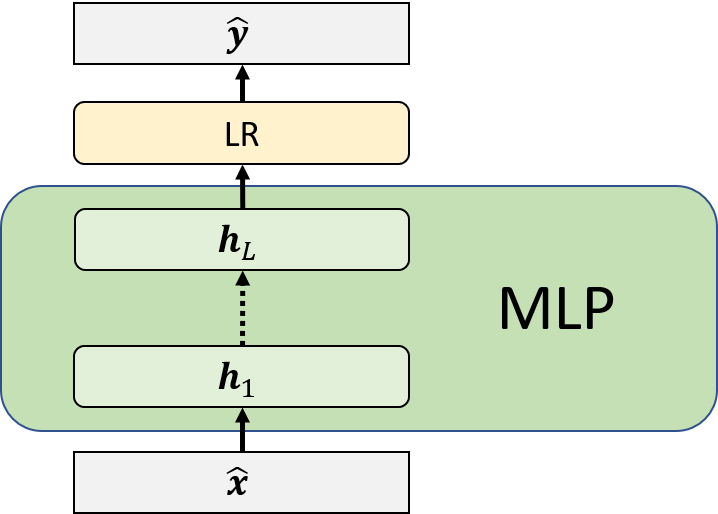
\includegraphics[width=.7\textwidth]{pics/dnn.png}
\caption{{\bf M}ulti-{\bf L}ayer {\bf P}erceptron}\label{fig:dnn}
\end{minipage}
\begin{minipage}{.04\textwidth}
\end{minipage}
\begin{minipage}{.48\textwidth}
  \centering
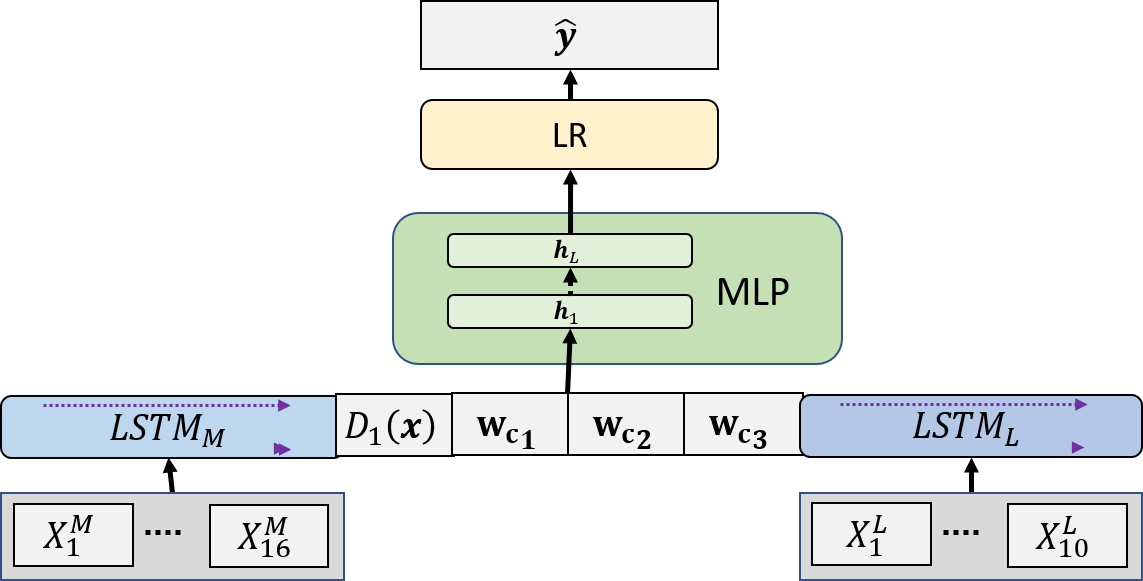
\includegraphics[width=\textwidth]{pics/rnn.png}
\caption{{\bf J}oint {\bf R}ecurrent {\bf N}eural {\bf N}etwork}\label{fig:rnn}
\end{minipage}
\end{figure}

For both the MLP and JRNN models, we use Dropout \citep{srivastava2014dropout} and Batch Normalization \citep{ioffe2015batch} to avoid overfitting and stabilize gradient updates respectively.
We fit the parameters of the JRNN, MLP, and LR models\footnote{Implemented in Tensorflow \citep{abadi2016tensorflow}. Code to be open sourced pre-publication.} by minimizing the cross-entropy
between the ground truth and predictions with the ADAM \citep{kingma2014adam} optimization algorithm. 

%============================================================================================
%Section: Results and Analysis================================================
%=============================================================================================
%============================================================================================
\section{Results and Analysis}
For each data subset, we trained model classes (RF, LR, MLP, JRNN) across 200 random configurations of their respective hyperparameters. 
Due to the limited amount of samples and wide ecological and environmental diversity across the study area, we used random 5-fold cross-validation splits (with equivalent joint distributions of ecoregion and coverage class) for each experimental run. 

Table \ref{tab:perf2} shows the average accuracy across cross-validation folds for the most accurate models trained on the 4 subsets of input variables.
Table \ref{tab:pscores} shows the p-values from one-tailed t-tests of accuracy improvement for models that incorporate satellite imagery. For all models, incorporating satellite data from either LandSat or MODIS provides significant gains in accuracy. LR and RF show more gains for LandSat than MODIS but no significant gains from using both platforms. While the deep learning models are ambivalent to finer time granularity (MODIS) or finer spatial granularity (LandSat) imagery, only the JRNN model gains significantly ($\alpha=0.1$) from multiple platforms. 
 
A principal outcome of this study is  a map of cheatgrass invasion estimates over the full study region. We dervived a final map \footnote{Contact kyle.larson@pnnl.gov for access to the final mapping product.} using a best-consensus mapping approach to combine each cross-validation prediction from the most accurate MLP model. We confirmed the utility of the map by expert review of sampled cheatgrass coverage predictions.  
\begin{figure}
\centering
 \begin{tabularx}{.87\linewidth}{l r r r r| r r r r }
		\toprule[.2em]		
		 &\multicolumn{4}{c|}{Mean Accuracy over Folds}&\multicolumn{4}{c}{Standard Deviation of Accuracy}\\
		&$D_1$& $D_2$&$D_3$&$D_4$&$D_1$&$D_2$&$D_3$&$D_4$\\
		\midrule
		{\bf LR}&76.712&79.611&81.215&{\bf 81.441}&0.021&0.019&0.019&0.012\\
		{\bf RF}&80.149 &81.667 &82.484&{\bf 82.794}&0.024&0.024& 0.022&0.025\\
		{\bf MLP}&79.604& 82.010&82.449 &\textcolor{red}{\bf 83.192}&0.025&0.014&0.015&0.012\\
		{\bf JRNN}&--- & 82.050&82.580&{\bf 83.184}&---&0.011&0.012&0.012\\
		\bottomrule[.2em]
	\end{tabularx}
	\captionof{table}{Classification accuracy of models for subsets of data} \label{tab:perf2}
  \end{figure}
\begin{figure}
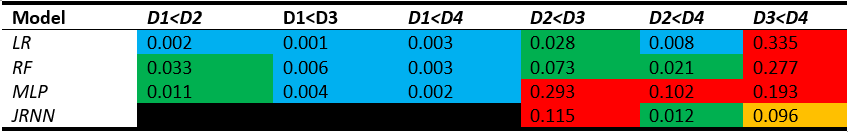
\includegraphics[width=\textwidth]{pics/pvalues.png}
	\captionof{table}{p-values from standard one-tailed t-test for improvement in accuracy. Colored cells denote passing a test for a particular $\alpha$ value. \crule[cyan]{8pt}{8pt} $\alpha=0.01$, \crule[green]{8pt}{8pt} $\alpha=0.05$, \crule[orange]{8pt}{8pt} $\alpha=0.1$, \crule[red]{8pt}{8pt} Not significant. } 
\label{tab:pscores}
\end{figure}
\section{Conclusion}
In this study we evaluated the efficacy of several machine learning approaches for mapping cheatgrass invasion, which poses significant risks to managing wildfire and environmental sustainability in the Western U.S.. %Furthermore, we sought to demonstrate the utility of these approaches for learning representations of cheatgrass from large, diverse datasets that are representative of the types of data that domain experts seek to fuse more effectively. 
Overall, the machine learning methods we tested were considered very successful at predicting cheatgrass occurrence (~76-83\% accuracy) for such a large and ecologically diverse area. %So-called “deep learning” methods yielded the best results, although competitive results were achieved with logistic regression and Random Forest. 
The accuracy of all four model types improved with the addition of time-series satellite data from two different platforms (MODIS Terra and Landsat-7), indicating they can effectively learn more discriminative representations of cheatgrass from large, multi-modal volumes of data.

We hope
the full region mapping product will aid in mitigating detrimental effects of cheatgrass invasion, and promote
new field studies for critical locations that may have heightened fire risk.
While this assessment of prospective machine learning models is specific to cheatgrass, it can also lend
insight and guidance to similar land cover mapping applications in the future, especially those requiring large volumes of data to adequately characterize phenomena over wide geographic regions. 

\subsubsection*{Acknowledgements}
We would like to thank the U.S. Fish and Wildlife Service (USFWS) for its support of related research that ultimately made this work possible, as well as those who kindly contributed field data including the USFWS, U.S. Geological Survey, Bureau of Land Management’s Inventory and Monitoring Program, Joint Base Lewis McChord-Yakima Training Center, and the SAGEMap\footnote{\url{http://sagemap.wr.usgs.gov}} and SageSTEP \footnote{\url{http://www.sagestep.org}} programs.
%This work was funded by the Deep Learning for Scientific Discovery Laboratory Directed Research and Development investment at the Pacific Northwest National Laboratory. 
%Pacific Northwest National Laboratory is operated for the U.S. Department of Energy by Battelle under Contract DE- AC05-76RL01830.
\bibliography{fiery}
\bibliographystyle{iclr2019_conference}

\end{document}
































